% !Mode:: "TeX:UTF-8"

\chapter{测试方法}

\section{后端接口测试}

本项目选择Postman作为测试工具,模拟前端的请求来进行后端接口的测试。下面的例子为对于新开发的评论功能中,由商家编号列出所有对于此商家评价信息接口的测试。

选择Post方法,请求时的参数采用x-www-form-urlencoded选项,对应信息头-application/x-www-from-urlencoded,会将表单内的数据转换为键值对。可以看到Http状态码为200OK,说明成功响应,最终后端响应的结果是一个包含所需信息的json对象。

\begin{figure}[H]
    \centering
    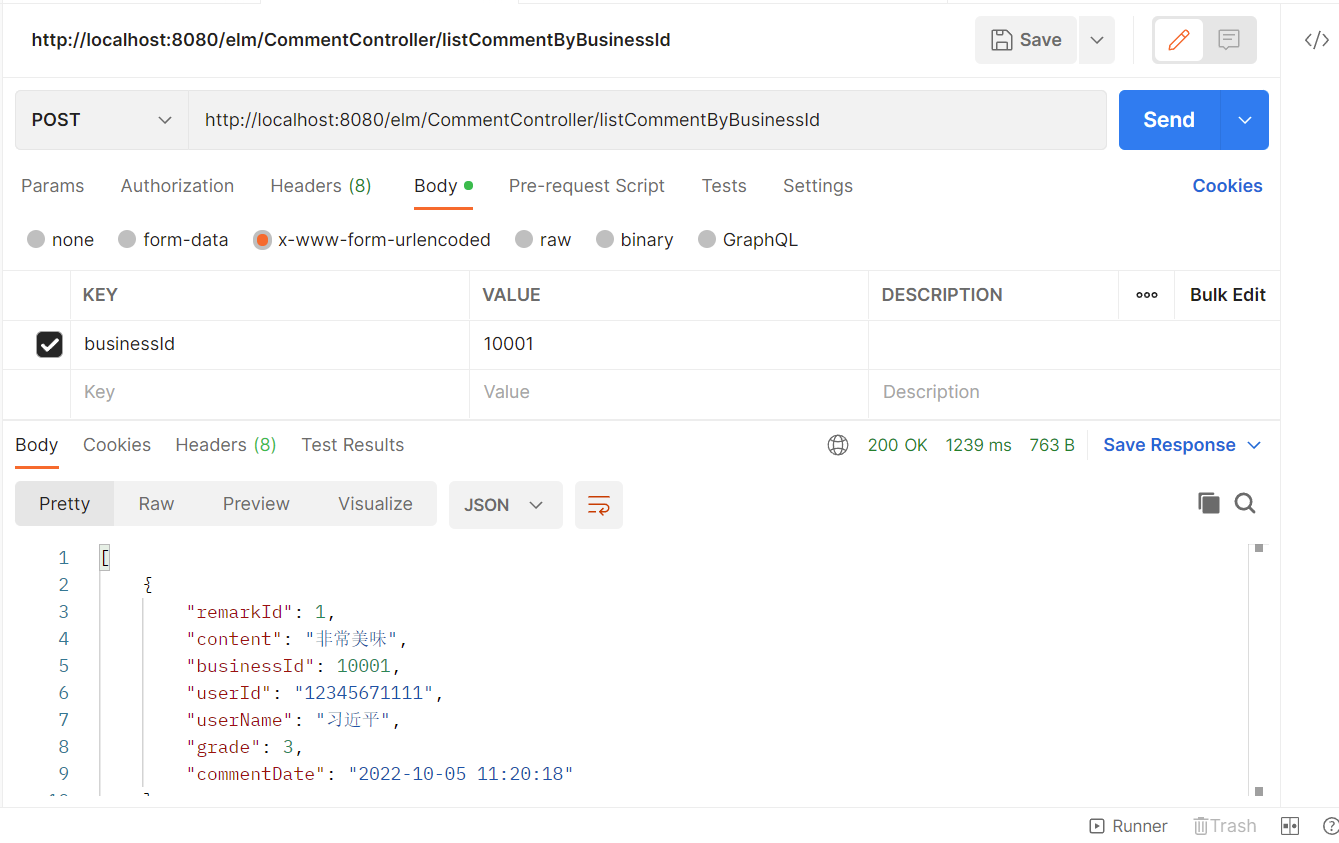
\includegraphics[scale=0.3]{figures/7.1.1.png}
    \caption{提交记录}
\end{figure}

\section{集成测试}
小组约定,当前后端分别完成本阶段的代码编写之后,各自将代码推到github上,再统一拉取做集成测试,在集成测试中,前后端合作debug,对于出现的bug先判断是前端还是后端的差错,再由对应成员做调试修改。







